\chapter{Related Work} % application of concepts
\label{chap:related-work}

% Try to highlight the differences between the state-of-the-art and your thesis. The goal is to:
% (a) do not re-invent the wheel, we can use major pillars of existing work to build upon
% (b) similarly, we do not want to propose something that is already existing. Thus, we need to show the "delta".

% not really any similar work available, therefore considering a larger scope and show the basis for my experimental setup:
As the whole field of NeuroStrike research and brain-computer interface simulations is very novel, there unfortunately does not exist any directly related work. To the best of our knowledge, no research regarding simulations of NeuroStrikes and potential mitigation approaches has been published. Therefore the scope of analysis for related work was expanded. \\
By following this approach, relevant literature could nonetheless be identified, and important findings and approaches derived. Especially previous work that is related to the simulation character of this research, was considered.\\
First, some \textit{models for the simulation of cognitive processes} were analyzed and compared, to ensure the relevance of later performed research on top of such a model. After that, the extended literature related to the \textit{simulation of NeuroStrikes} was considered. 


\section{Models for the Simulation of Cognitive Processes}
% as concise as possible, documentation of the models I compare
    In the first step, it is essential to choose a suitable Model for the simulation of a cognitive process. For a model to be suitable in the context of this work, it has to adhere to some key criteria, specifically:
    \begin{enumerate}
        \item It has to represent a brain area, that is \textbf{related} to a cognitive process and affected by NeuroStrike attacks.
        %(The Amygdala or Hippocampus and their associated processes of fear/anxiety respectively memory/learning are of special interest, as they are best related to the effects of NeuroStrikes (reference?)).
        \item It has to allow for the simulation of the cognitive process in a \textbf{meaningful} and measurable way.
        \item The model and its associated simulator have to facilitate the \textbf{integration} of the attack and its countermeasure into the simulation.
        \item It should be as \textbf{realistic} as possible.
    \end{enumerate}

    Based on the literature presented in the previous sections and the first criteria, the search for potential models was directed towards ones of the hippocampus and amygdala. Furthermore, the "NEST" \cite{Gewaltig:NEST}, "NEURON" \cite{Hines.1997}, and "Brian2" \cite{Stimberg.20.8.2019} simulators (introduced above), were deemed to be the most suitable options for the given research conditions, which also guided the preliminary selection. The search for potential models was conducted on ModelDB \cite{McDougal.2017} and the most promising ones identified there are followingly analyzed in depth and compared in the end.

    \subsection{A 1000 cell network model for Lateral Amygdala}
    % https://modeldb.science/150288
    This model represents the dorsal part of the lateral amygdala (LA) and was written for the NEURON simulator. It was created to assess the importance of different factors that play a part in fear conditioning. The evaluated factors were: the increased responsiveness of neurons projecting to the LA, their synapses' plasticity, and LA internal synapses' plasticity. To monitor their effect on fear conditioning, they observed the temporal pattern of the neurons increase in tone responsiveness \cite{Kim.2013}, which is associated with fear conditioning \cite{Repa.2001}. \\
    It is a bio-physically realistic model which is scaled down in a ratio of 30:1. Therefore consisting of 1'000 neurons (800 principal cells and 200 interneurons), which are connected by almost 40'000 synapses. The neurons were modeled with multiple compartments (cell body and one or two dendrites) and different spiking frequencies (for the principal cells). Due to the high number of neurons, they were distributed randomly in a 3-dimensional space and connected based on some observed general rules and their derived probabilities. On average resulting in about 60 excitatory and 20 inhibitory inputs per principal cell. Component-wise adjustments were impossible for the model tuning and validation process, due to its scale. Nonetheless, it managed to reproduce the expected high-level behavior precisely, even though it is mostly based on low-level details. \\
    Regarding the input, the model incorporates the simulation of thalamic and cortical inputs via glutamatergic synapses acting on AMPA/NMDA receptors (at 20 or 40 Hz). But also random excitatory background inputs to all model cells \cite{Kim.2013}.

    \subsection{Model of CA1 activity during working memory task}
    % https://modeldb.science/223962
    This is a model that represents some neurons of the hippocampus, specifically pyramidal cells from the CA1 region. It was also written for the NEURON simulator and created to investigate working memory capacity (WMC) on the single neuron level. The WMC was analyzed in the context of a delayed free recall task, where a certain amount of items from a list must be recalled. To quantify the performance, the cumulative latency of this free recall was taken as a benchmark. Lower latency values are associated with higher WMC, whereas higher values suggest the opposite. \\
    The simplifying assumption was made, that a single neuron of the hippocampus could code for an object and would fire if it was presented with the according stimuli of the sensory systems. On a structural level, that meant that each neuron was modeled the same, with 26 oblique dendrites, originating from the cell body. Each dendrite conceptually represents a feature, which allows the neuron to encode for objects, by responding to certain combinations of these. During the simulation, random groups of 1 to 26 dendrites were then stimulated with synaptic inputs, while a level of realistic background synaptic activity was maintained. This background activity balanced to achieve an average resting potential of -65 mV. The number of neurons simulated was matched to the number of words that should be recalled, resulting in the simultaneous simulation of 6, 9, or 12 neurons. \\
    The main adjustable parameters of the model are the amount of dendrites that are being stimulated, as well as the level of background noise. The dendritic location of the synapses, as well as the pattern of background activity, was randomized across simulations \cite{Spera.2016}.
    
    
    \subsection{Model of the hippocampus over the sleep-wake cycle using Hodgkin-Huxley neurons}
    % https://modeldb.science/243350
    This is a detailed model, which represents the hippocampus as well as the entorhinal cortex in an anatomically accurate fashion. It was written for the Brian2 simulator in Python to analyze the effects of different changes in the network that appear during the sleep-wake cycle. Especially the role of varying acetylcholine concentrations during these cycles was explored, by simulating their modulatory effect on the functional connectivity of the hippocampus. To quantify the results, the output (in the form of extracellular recordings) was analyzed and compared to the expected oscillatory rhythms. \\
    Each neuron was simulated according to Hodgkin-Huxley's model as single-compartment and conductance-based. Principal excitatory neurons were modeled as pyramidal cells with sodium, potassium, and calcium ion channels. Some of them also received a Calcium-Activated-Nonspecific (CAN) cationic channel. Interactions between neurons were modeled with excitatory and inhibitory synapses. In total over 30'000 neurons were used to represent the hippocampal formation and entorhinal cortex. The hippocampal formation was further divided into the "dentate gyrus", CA1, and CA3, where the amount and type of neurons in each structure were adjusted to match values suggested by the literature. But also the whole spatial organization was matched to the human anatomy as shown in Figure \ref{fig:hippocampus-model}. The importance and benefits of this have been shown by \textcite{Aussel.2018}, who compared its performance against less realistic topologies and connectivity settings.
    \begin{figure}[H]
        \centering
        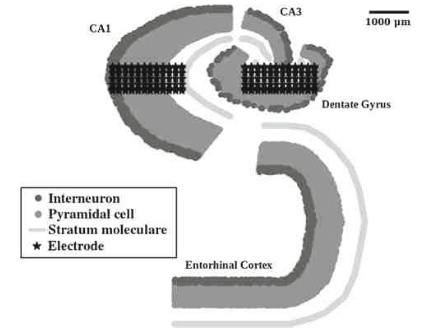
\includegraphics[width=0.45\linewidth]{images/hippo-model-brian2.png}
        \caption{Topology of the Model \cite{Aussel.2018}}
        \label{fig:hippocampus-model}
    \end{figure}
    The external input is only inserted at the neurons of the entorhinal cortex and then propagated to the other structures from there. To represent inputs from the rest of the brain as realistic as possible, each input neuron is stimulated by a variable firing rate, derived from real recordings of sleep/wake SEEG signals. Furthermore, the model offers many conductance-related and general parameters that can be adjusted \cite{Aussel.2018}. 
    

    \subsection{Comparison and Conclusion}
    % Show table of compared models and mention and justify the selected model based on information supplied
    Considering these models under the criteria mentioned at the beginning of the section, the \textit{model of the hippocampus} turned out to be most suited for use in this thesis.\\
    Whilst the model of the \textit{lateral amygdala} did not allow for a strong enough relation to the performance of a high-level cognitive process, the one concerned with \textit{working memory capacity} lacks the necessary realism. Even though every neuron is modeled realistically, its limited network size makes inferences on complex cognitive processes difficult.\\
    The model of the \textit{hippocampus} on the other hand, adheres fairly well to all the criteria. It provides a clear and measurable relationship to learning and memory, by observing certain activity patterns. Furthermore, it supplies a large parameter space, which should facilitate the integration of the electromagnetic attack. Lastly, modeling as many neurons as it does, in a spatially accurate manner, makes it the network-wise most realistic option.
    


\section{Simulation of Neurostrikes}
% What work has been done, regarding the Attacks
    To simulate the impact of neurostrike on the brain, their exact effects on the brain need to be explored and understood. This section therefore is dedicated to assessing the state of the art when it comes to the simulation of such attacks and their underlying mechanisms. But as the whole topic of neurostrikes is novel and to a certain degree still disputed, not much literature can be found regarding its mechanisms and effects. Let alone any work of attack simulations in functional brain simulations. Therefore, this section is concerned with summarizing and discussing, what has been proposed by the current literature on neurostrikes. Filling the gaps where necessary with findings in the field of electromagnetic radiation, as it is considered the underlying technology. This shall then serve as a basis for integrating such an attack into the simulation and ultimately guide the design of a countermeasure.

    
    \subsection{Neurostrikes}
    % Based on what I simulate the attacks (NeuroStrikes) - specific effects of NeuroStrikes on the Brain (and area of the cognitive process)
    To ensure that the relation between the attack and cognitive warfare is maintained as well as possible, the available specific literature (even though sparse) will set the general frame for its implementation. Therefore the \textit{Havana Syndrome}, being the best-documented case of its potential occurrence and effects, will be analyzed first. The focus is set on the related symptoms as more specific elaborations are difficult without making assumptions about its underlying mechanism (which shall be reserved for the subsequent section).
    
    The symptoms that were reported in cases of the Havana syndrome, can be split into ones that occurred during the \textit{initial} and sudden onset of the illness, as well as \textit{persisting} or recurring ones.\\
    The \textbf{initial} symptoms were reported to mostly start with the perception of a loud sound, described as clicking or screeching, accompanied by a strong feeling of vibration or pressure and pain in the head. Interestingly most victims described these sensations to come from a specific direction. Less often were the reports of tinnitus, hearing loss, dizziness, unsteady gait, or visual disturbances.\\
    The \textbf{persisting} or long-term effects include some similar symptoms, but for the most part, are distinct. Dizziness for example is something that persisted in many individuals, but also headaches became chronic in some patients. Further reported symptoms include: fatigue, impaired balance, concentration, and memory, but also depression and insomnia \cite{Pavlin.2020}.
    

    \subsection{Electromagnetic Radiation}
    % since only little literature is available; supplement with research regarding "pulsed RadioFrequency Electromagnetic waves" and their effects
    To the best of our knowledge, also no previous work exists on simulating Electromagnetic attacks or EMR in general, inside a functional model of the brain or any substructure. Therefore, this section will discuss general findings and proposals, for the effects of EMR on the brain. A special focus will be laid on the supposed underlying technology of NeuroStrikes, pulsed RF EMR. But also general findings regarding EMR will be included to supplement the sparse literature. It should be mentioned that most of these findings were made through animal experiments and that the results are by no means uniform.

    % 1. electromagnetic radiation has effects on brain
        % Many studies indicate effect: Zhi.2017
        % Treshold intensity: DAndrea.1999
        A large body of literature suggests that EMR can have a series of negative effects on the brain and its function \cite{Hu.2021} \cite{Lai.1994} \cite{Zhi.2017}. However, the specific effects on the brain can differ, depending on a few radiation exposure parameters. For example, it may require a certain irradiation intensity threshold to be reached, before significant changes appear at all \cite{DAndrea.1999}. Whilst for RF radiation, their modulation into pulses seems to be essential \cite{Huber.2005}. But also the radiation frequency in general and its power plays an important role, as changes in these parameters can lead to alterations of the observable effects \cite{Hu.2021}.
        
    % 2. changes of activity, damage to brain areas, neurotransmitter changes
        % General: Tan.2017
        % Highlevel effects: Anxiety - Kereya.2018, Headache/memory - Lin.2021
        % Neurotransmitter changes: Acetylcholine increase - Kumar.2016
        From a \textbf{high-level} (functional) perspective, \textbf{effects} include the emergence of fear or anxiety \cite{Kereya.2018}, but also impairments of learning, memory, headaches, and more \cite{calvente2016does} \cite{Lin.2021} \cite{Tan.2017}. This is similar to the functional impairments that are associated with NeuroStrikes. Specifically considering the reports related to the Havana syndrome, as presented above.\\
        Regarding \textbf{lower-level effects} of EMR and potential causes of these functional impairments, different alterations in the brain have been observed. However, the focus was set according to the simulation model choice and directed towards the hippocampus and memory impairments.\\ % Insert more details if necessary
        One category of identified alterations was \textit{structural damage} to certain brain areas \cite{Hu.2021} \cite{Tan.2017}, for example, the hippocampus and cerebral cortex \cite{Lin.2021}.\\
        Furthermore, a wide range of \textit{neurotransmitter changes} were recorded in the context of EMR. Including alterations in dopamine, serotonin, norepinephrine, and acetylcholine levels \cite{Hu.2021}.\\
        But changes in general \textit{electrophysiological activity} have also been reported, specifically after exposure to RF EMR. Some experiments for example showed that the majority of irradiated cells reduce their spontaneous activity \cite{seaman1978slow} \cite{wachtel1975effects}. Others identified differences between initial and long-term effects, where the excitability of the neurons is increased in the beginning and only reduced after longer exposures \cite{dumansky1974biologic}.

    % 3. radio frequency effect on hippocampus and amygdala
        % General: Lai.1994, Narayanan.2019
    
    \subsection{Conclusion and derived parameters}
    The literature supplies a lot of indications that NeuroStrikes and specifically RF EMR, do impair the cognitive processes of memory and learning. A few underlying changes could further be identified to be the most promising cause for that. First of all, the structural damage to the hippocampus, as this structure plays an important role in the cognitive process. But also changes in the neurotransmitter acetylcholine could be responsible for the disturbance of those processes, as they play a key role in their modulation \cite{Aussel.2018}.
    

\section{Research Gap and Motivation}
% Clear identification of Knowledge gap in the literature 
    % -> Underlying Mechanisms of Neurostrikes
    % show with table
To conclude the review of related work, that was performed in this chapter, an overview of the available literature will be performed in this section. This shall summarize what has been done, and allow for a clear identification of the research gap. In the following, the available resources and literature on the simulation of cognitive processes are evaluated, before a more detailed analysis is performed on the works related to NeuroStrikes.

    \subsection{Simulation of Cognitive Processes}
    In the realm of brain simulators and works that are related to them, it was possible to identify a series of resources that fulfill the general requirements for this work. Showing that there exist simulation models, that combine a realistic topology with the capability to represent the performance of a cognitive process. As specified in the according section, some of the investigated models, are better suited than others. Especially because such complex models, incorporate many aspects, that need to fit the specific use case. The available resources do however cover the simulation field of interest sufficiently, which allows this work to focus its research on other aspects. 
    

    \subsection{Simulation of NeuroStrikes}
    A goal of this work is, to integrate a NeuroStrike (or Electromagnetic attack) into the simulation of the cognitive process. As however already discussed in the dedicated chapter above, the literature on NeuroStrikes is sparse. Especially regarding any specific explorations of their effect on the brain. It is, therefore, no surprise that even less literature, respectively none at all, could be identified, that integrates such an attack into a simulation. The alternative approach, investigating the most probable underlying technology of NeuroStrikes (RF EMR), has also been elaborated in more detail.

    \begin{table}[htbp]
        \centering
        \caption{Overview of existing work on NeuroStrikes and their mechanism}
        \begin{tabular}{@{}m{3cm} m{2.5cm} m{4cm} m{5cm}@{}}
            \toprule
            \textbf{Context} & \textbf{Reference} & \textbf{Investigated Aspects} & \textbf{Findings} \\ 
            \midrule
        \end{tabular}
        \renewcommand{\arraystretch}{1.3}
        \begin{tabular}{@{}p{2.9cm} p{2.5cm} p{4cm} p{5cm}@{}}
            NeuroStrikes 
                & \small{\textcite{McCreight.2024}} & \small{general assessment} & \small{high relevance, related to nano pulsed RF EMR} \\
                & \small{\textcite{EADS.2023}} & \small{general assessment} & \small{high relevance, causes cognitive impairments through \newline series of technologies} \\ 
                & \small{\textcite{McCreight.2022}} & \small{symptoms and potential causes} & \small{many symptoms, caused by RF EMR} \\
                & \small{\textcite{Pavlin.2020}} & \small{symptoms, potential causes, and brain \newline alterations} & \small{wide range of acute and persistent symptoms, likely caused by RF EMR, showing unspecific brain damage} \\ 
        \midrule
            Electromagnetic Radiation
                & \small{\textcite{Narayanan.2019}} & \small{symptoms} & \small{can cause range of symptoms} \\
                & \small{\textcite{Zhi.2017}} & \small{symptoms and brain \newline alterations} & \small{many mechanisms involved in cognitive impairments} \\ 
                & \small{\textcite{Tan.2017}} & \small{symptoms and brain \newline alterations} & \small{many mechanisms lead to memory impairments} \\ 
                & \small{\textcite{Lai.1994}} & \small{brain alterations} & \small{overview of many effects on the brain} \\
                & \small{\textcite{Lin.2021}} & \small{brain alterations} & \small{neurotransmitter changes and damage in hippocampus} \\
                & \small{\textcite{Hu.2021}} & \small{brain alterations} & \small{influence on many neurotransmitters} \\
                & \small{\textcite{Fujiwara.1978}} & \small{brain alterations} & \small{large increase in acetylcholine} \\
                & \small{\textcite{Shahin.2015}} & \small{brain alterations} & \small{increased cell apoptosis} \\ 
                & \small{\textcite{Altun.2017}} & \small{brain alterations} & \small{large decrease in neurons} \\ 
                & \small{\textcite{Xu.2006}} & \small{brain alterations} & \small{damage to synapses in \newline hippocampus} \\ 
            \bottomrule
        \end{tabular}
        \label{tab:neurostrike-literature}
    \end{table}
    % No literature exploring, how Neurostrikes affect the brain on a low level
        % and thereby induce the associated symptoms
    % Motivation for my research contribution
    This section aims to provide a better overview of the literature that was considered throughout the review, to illustrate the identified research gap. For this purpose, table \ref{tab:neurostrike-literature} was created, stating the investigated aspects and specifying their findings. The entries are primarily sorted by the context of the literature, which already reveals the obvious lack of NeuroStrike-related work. Inside of each context, the sources are then ordered according to the specificity of their research.\\
    This shows that from the little literature that exists on NeuroStrikes specifically, only one considers its impact on the brain. The there identified brain alterations are however neither extensive nor very specific. Most are concerned with a more general assessment of the topic and mention only high-level effects like symptoms of the attacks.\\
    What exactly happens inside the brain of an attacked victim, that leads to such symptoms, remains therefore unclear and was identified as the most relevant research gap of this work.

    As table \ref{tab:neurostrike-literature} shows, it was however possible to identify a lot more work regarding RF EMR, and its low-level effects on the brain. This motivated the following simulation research, during which such effects will be integrated into the model, to evaluate whether they could be responsible for NeuroStrike symptoms. Thereby striving to validate the connection between RF EMR and NeuroStrikes and lay a foundation for the simulation of such attacks.

    
    